\section{$\forall$-step}

\begin{frame}{Linear Plans are Bad!}
Consider the following (single) planning problem:
\begin{center}\begin{tikzpicture}[scale=1.0]
    \tikzstyle{N}=[draw,circle,minimum size=4pt,inner sep=0pt]
	
	\node[N,blue] (A1) at (0,0) {C};
	\node[N] (A2) at (2,0) {B}; \node at (2.5,0) {\faArchive};
	\node[N] (A3) at (1,2) {A}; \node at (0.5,2) {\faTruck};
	\draw (A1) -- (A2);
	\draw (A2) -- (A3);
	\draw (A3) -- (A1);
	
	\node[N] (B1) at (5,0) {F}; \node at (4.5,0) {\faTruck};
	\node[N,blue] (B2) at (7,0) {E};
	\node[N] (B3) at (6,2) {D}; \node at (6.5,2) {\faArchive};
	\draw (B1) -- (B2);
	\draw (B2) -- (B3);
	\draw (B3) -- (B1);
 \end{tikzpicture}\\[\baselineskip]
\pause
\scalebox{0.8}{$\text{drive}(A,B), \text{load}(B), \text{drive}(B,C), \text{unload}(C), \text{drive}(F,D), \text{load}(D), \text{drive}(D,E), \text{unload}(E)$}\\[\baselineskip]
\pause
	\scalebox{0.8}{\begin{tabular}{l l l l}
		drive$(A,B)$ & load$(B)$ & drive$(B,C)$ & unload$(C)$\\
		drive$(F,D)$ & load$(D)$ & drive$(D,E)$ & unload$(E)$
	\end{tabular}}
\end{center}
\end{frame}





\begin{frame}{$\forall$-step [Kautz\&Selman, AAAI'96]}
\begin{center}
	Allow parallel execution of actions.\qquad But when?
\end{center}
\pause
\begin{itemize}[<+->]
    \item Let $\mathcal A$ be some set of actions.
	\item Parallel execution of $\mathcal A$ is safe, if all ($\forall$) linearisations of $\mathcal A$ are executable.% (Note the similarity to POCL planning.)
	\item Necessary conditions:
	\begin{itemize}
		\item All actions are executable in the previous state as all could be the first.
		\item No action can have a delete-effect that is a precondition of another action, i.e., $\forall a_1 \neq a_2 \in \mathcal A: del(a_1) \cap prec(a_2) = \emptyset$, as $a_1$ can occur directly before $a_2$.
	\end{itemize}
	\item Sufficient conditions: \visible<7->{Necessary conditions are already sufficient.}
\end{itemize}
\vspace{0.3cm}
\visible<8->{Further requirements for nice encoding?}\\
\visible<9->{The resulting state must unique!}\\
\visible<10->{We forbid two actions $a_1,a_2$ with $del(a_1) \cap add(a_2) \neq \emptyset$ to be executed in parallel.}\\
\visible<11->{We don't have to model this: $a_1^t \implies \neg v^t \wedge a_2^t \implies v^t$ imples $\neg a_1^t \lor a_2^t$.}
\end{frame}






\begin{frame}{Encoding $\forall$-step}
\hspace*{-.3cm}\Wider{1.04}{
    Remove the at-most-one constraints and add:\\[-2.5em]\pause

	\begin{align*}
		a_1^t \rightarrow \neg a_2^t \quad \quad \forall a_1,a_2 \in A\text{ with } del(a_1) \cap pre(a_2) \neq \emptyset
	\end{align*}\ \\[-2em]
	\centering $\rightarrow$ quadratic effort.\pause\\
	\vspace{1cm}Is this the best we can do? \pause \alert{No!}
	}
\end{frame}



\begin{frame}{Encoding Interference}
\textbf{Idea 1}: switch from a action-centric to a state variable-centric view.\\
\qquad \visible<2->{For every $v \in V$: if $v \in add(a_1)$ and $v \in del(a_2)$ add $a_1^t \rightarrow \neg a_2^t$}\\
\visible<3->{\textbf{Idea 2}: if one action with $v \in del(a_2)$ is forbidden, so are all others.}\\
\visible<4->{\textbf{Idea 3}: express this with additional variables!}\\
\visible<5->{The only problem is that an operation must not disable itself.}\\
\vspace{0.3cm}
\visible<6->{Arrange the actions with $v \in pre(a) \cup del(a)$ as a sequence $S$.}\\[0.2cm]
\visible<7->{\begin{tabular}{lllllllllllllll}
$a_1$ & $a_2$ & $a_3$ & $a_4$ & $a_5$ & $a_6$ & $a_7$ & $a_8$ & $a_9$\\
\visible<8->{E &E&E& &E& & & E&E}\\
\visible<8->{R &R&  &R&R&R&R&&R&}\\
\end{tabular}
}
\vspace{0.4cm}
    \begin{itemize}
      \item<8-> $E_v$ -- subsequence of $S$ with $v \in del(a)$ (\textbf{E}rasing)
      \item<8-> $R_v$ -- subsequence of $S$ with $v \in pre(a)$ (\textbf{R}equiring)
    \end{itemize}
\end{frame}

\begin{frame}{Chains}
\begin{tikzpicture}
    \node<1->[] at (0,-0.0) {E};
    \node<1->[] at (1,-0.0) {E};
    \node<1->[] at (2,-0.0) {E};
    \node<1->[] at (4,-0.0) {E};
    \node<1->[] at (7,-0.0) {E};
    \node<1->[] at (8,-0.0) {E};

    \node<1->[] at (0,3.0) {R};
    \node<1->[] at (1,3.0) {R};
    \node<1->[] at (3,3.0) {R};
    \node<1->[] at (4,3.0) {R};
    \node<1->[] at (5,3.0) {R};
    \node<1->[] at (6,3.0) {R};
    \node<1->[] at (8,3.0) {R};

    \node<1->[P,label={\tiny\ensuremath{a_1}}] (A1) at (0,1.5) {};
    \node<1->[P,label={\tiny\ensuremath{a_2}}] (A2) at (1,1.5) {};
    \node<1->[P,label={\tiny\ensuremath{a_3}}] (A3) at (2,1.5) {};
    \node<1->[P,label={\tiny\ensuremath{a_4}}] (A4) at (3,1.5) {};
    \node<1->[P,label={\tiny\ensuremath{a_5}}] (A5) at (4,1.5) {};
    \node<1->[P,label={\tiny\ensuremath{a_6}}] (A6) at (5,1.5) {};
    \node<1->[P,label={\tiny\ensuremath{a_7}}] (A7) at (6,1.5) {};
    \node<1->[P,label={\tiny\ensuremath{a_8}}] (A8) at (7,1.5) {};
    \node<1->[P,label={\tiny\ensuremath{a_9}}] (A9) at (8,1.5) {};

	\node<2->[S] (E1) at (0.5,2.5) {};
	\node<2->[S] (E2) at (2.5,2.5) {};
	\node<2->[S] (E3) at (3.5,2.5) {};
	\node<2->[S] (E4) at (4.5,2.5) {};
	\node<2->[S] (E5) at (5.5,2.5) {};
	\node<2->[S] (E6) at (7.5,2.5) {};
	\draw<3->[->] (A1) -- (E1) {};
	\draw<3->[->] (A2) -- (E2) {};
	\draw<3->[->] (A3) -- (E2) {};
	\draw<3->[->] (A5) -- (E4) {};
	\draw<3->[->] (A8) -- (E6) {};
	\draw<4->[->] (E1) -- (E2) {};
	\draw<4->[->] (E2) -- (E3) {};
	\draw<4->[->] (E3) -- (E4) {};
	\draw<4->[->] (E4) -- (E5) {};
	\draw<4->[->] (E5) -- (E6) {};
	\draw<5->[->,red,thick] (E1) -- (A2);
	\draw<5->[->,red,thick] (E2) -- (A4);
	\draw<5->[->,red,thick] (E3) -- (A5);
	\draw<5->[->,red,thick] (E4) -- (A6);
	\draw<5->[->,red,thick] (E5) -- (A7);
	\draw<5->[->,red,thick] (E6) -- (A9);



	\node<6->[S] (F1) at (0.5,0.5) {};
	\node<6->[S] (F2) at (1.5,0.5) {};
	\node<6->[S] (F3) at (3.5,0.5) {};
	\node<6->[S] (F4) at (4.5,0.5) {};
	\node<6->[S] (F5) at (5.5,0.5) {};
	\node<6->[S] (F6) at (6.5,0.5) {};
	\draw<6->[->] (A9) -- (F6) {};
	\draw<6->[->] (A8) -- (F6) {};
	\draw<6->[->] (A5) -- (F3) {};
	\draw<6->[->] (A3) -- (F2) {};
	\draw<6->[->] (A2) -- (F1) {};
	\draw<6->[->] (F2) -- (F1) {};
	\draw<6->[->] (F3) -- (F2) {};
	\draw<6->[->] (F4) -- (F3) {};
	\draw<6->[->] (F5) -- (F4) {};
	\draw<6->[->] (F6) -- (F5) {};
	\draw<6->[->,red,thick] (F1) -- (A1);
	\draw<6->[->,red,thick] (F2) -- (A2);
	\draw<6->[->,red,thick] (F3) -- (A4);
	\draw<6->[->,red,thick] (F4) -- (A5);
	\draw<6->[->,red,thick] (F5) -- (A6);
	\draw<6->[->,red,thick] (F6) -- (A7);

    \node<7->[P,blue] at (A3) (2,1.5) {};
	\node<7->[S,blue] at (E2) {};
	\node<7->[S,blue] at (E3) {};
	\node<7->[S,blue] at (E4) {};
	\node<7->[S,blue] at (E5) {};
	\node<7->[S,blue] at (E6) {};
	\node<7->[S,blue] at (F1) {};
	\node<7->[S,blue] at (F2) {};


    %\node<1->[P,label={[below,label distance =-0.3cm]\tiny\ensuremath{a_2}}] (A2) at (1,1) {};
    %\node<1->[P,label={\tiny\ensuremath{a_5}}] (A3) at (1,2) {};
    %\node<1->[P,label={\tiny\ensuremath{a_4}}] (A5) at (2,2) {};
    %\node<1->[P,label={[below,label distance =-0.3cm]\tiny\ensuremath{a_3}}] (A4) at (2,1) {};
    %\draw<1->[->] (A1) -- (A2);
    %\draw<1->[->] (A3) -- (A1);
    %\draw<3->[->,red] (A3) -- (A1);
    %\draw<1->[->] (A3) -- (A2);
    %\draw<3->[->,red] (A3) -- (A2);
    %\draw<1->[->] (A2) -- (A4);
    %\draw<1->[->] (A4) -- (A5);
    %\draw<1->[->] (A5) -- (A3);

\end{tikzpicture}
      \visible<8->{\begin{align*}
        chain(E&,R) = \\
		\bigwedge &\{a^i \rightarrow \mathtt{f}^j \mid i < j, a_i \in E, a_j \in R, \{a_{i+1}, \dots, a_{j-1}\} \cap R = \emptyset\} \cup {}\\
        &\{\mathtt{f}^i \rightarrow \mathtt{f}^j \mid i < j, \{a_i, a_j\} \in R, \{a_{i+1}, \dots, a_{j-1}\} \cap R = \emptyset\} \cup {}\\
      &\{\mathtt{f}^i \rightarrow \neg a_i \mid a_i \in R\}
      \end{align*}}
\visible<9->{Two chains for every $v \in V$ with \alert{fresh} decision variables $\texttt{f}^i$.}
\end{frame}




